% Wer Debian hat, kann LaTeX mit diesem Befehl installieren:
%  apt-get install  texlive texlive-lang-german texlive-latex-extra \
%  texlive-pictures texlive-science texlive-fonts-extra
% pdf generieren unter Linux:
%  pdflatex --output-directory /tmp/ langfassung-template.tex

% Diese Vorlage dient als Hilfestellung bei der Erstellung der schriftlichen
% Arbeit (die sogenannte Langfassung). Du bist nicht verpflichtet sie zu nutzen.
% Sie wurde zur Verf"ugung gestellt von Thomas@Wirsings.eu
%
% Die angef"uhrten Fragestellungen und Kommentare dienen nur als Anregung oder
% Checkliste, was bei einer Jugend forscht Arbeit beachtet werden sollte. Sie
% m"ussen nicht alle beantwortet werden. Weitere Hinweise findest Du im
% "Leitfaden zum Verfassen der schriftlichen Arbeit'' auf unserer Internetseite:
% www.jugend-forscht.de/teilnahme/ablauf/schriftliche-arbeit.html.
%
% Die Angaben zur Seitenanzahl dienen nur als grobe Orientierung, welchen Umfang
% die einzelnen Teile haben k"onnen.
%
% Du kannst Deinen Text einfach unter die Gliederungspunkte schreiben und daf"ur
% die Leitfragen und Kommentare l"oschen. Das Commando "\tbd" kann man nutzen um
% Teile zu markieren die noch nicht fertig sind.

\documentclass[10pt,twoside]{article}  % darf nicht kleiner sein (Vorgabe JuFo)
\pagestyle{headings}
\pagenumbering{Roman}
\usepackage[ngerman]{babel}
\usepackage[hidelinks]{hyperref}
\usepackage[a4paper]{geometry}
\usepackage{datetime}
\usepackage{graphicx}
\usepackage{color}
\usepackage[T1]{fontenc}
\usepackage[utf8]{inputenc}
\usepackage{charter}
\usepackage{tabularx}
\newcolumntype{C}[1]{>{\centering\arraybackslash}p{#1}}
\geometry{left=25mm,right=25mm, top=25mm, bottom=20mm}
  % R"ander bitte nicht kleiner (Vorgabe JuFo)
\setlength{\parindent}{0mm}

\newcommand{\tbd}[1]{\textcolor{red}{\large \bf tbd: #1}}

\begin{document}
  \title{\tbd{Title des JuFo-Projekts}}
  \setlength{\parskip}{0ex}
  \date{\today \ \currenttime \ MEZ}
  \maketitle
  \begin{center}
    \tbd{Titlebild}
    % 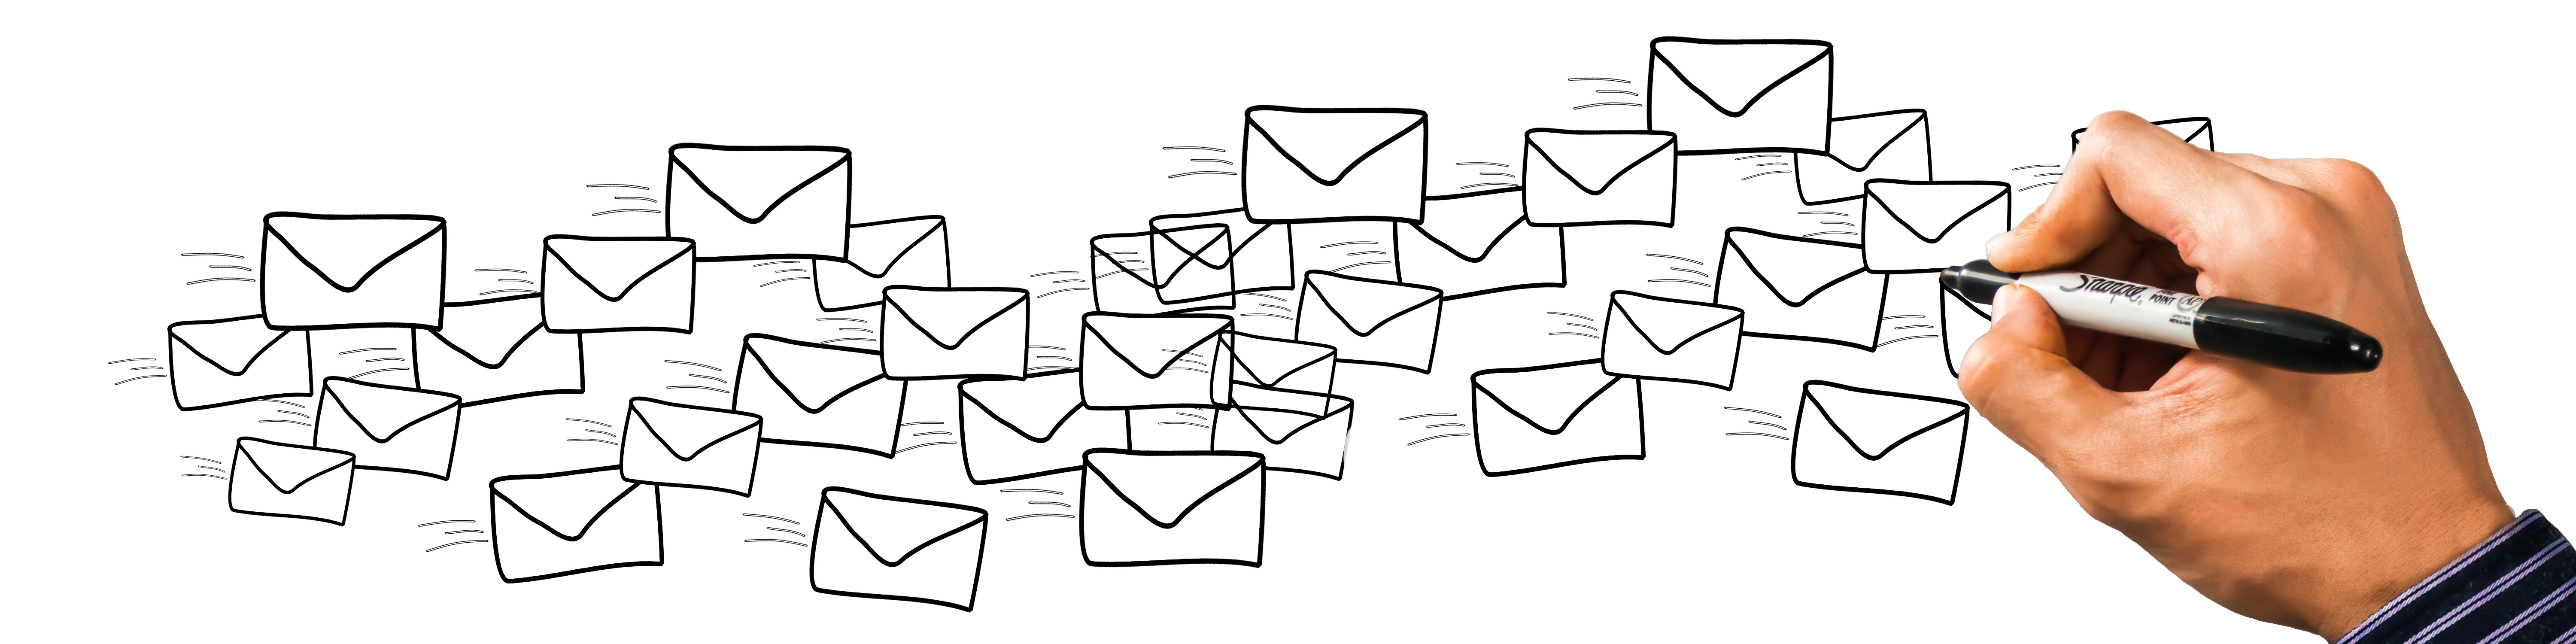
\includegraphics[width=1\textwidth]{Titelbild.jpg}
  \end{center}

  \hrulefill

  \tbd{Kurzfassung: Bitte in 6 bis 8 S"atzen beschreiben: Ziel des Projekts,
    Fragestellung, Vorgehensweise, Ergebnis} % 1/2 Seite

  \hrulefill

  \vfill
  \begin{tabular}{C{0.5\textwidth}C{0.5\textwidth}}
    \textbf{\tbd{Name 1}}    & \textbf{\tbd{Name 2}} \\
    \textbf{\tbd{Stra"se 1}} & \textbf{\tbd{Stra"se 2}} \\
    \textbf{\tbd{Ort 1}}     & \textbf{\tbd{Ort 2}} \\
    \textbf{\tbd{Email 1}}   & \textbf{\tbd{Email 2}} \\
  \end{tabular}
  \vfill

  \hrulefill

  \parbox{\textwidth}{\centering \bf Jugend-Forscht 20\tbd{XX} ---
    Regionalwettbewerb \tbd{Ort} --- \tbd{Fachbereich}}
  \thispagestyle{empty}
  \newpage

  \tableofcontents
  \listoffigures
  \listoftables
  \setlength{\parskip}{1ex}
  \cleardoublepage
  \pagenumbering{arabic}

  % ab hier max 15 Seiten % (Vorgabe JuFo)

  \section{Einleitung und Ziel} % 1 bis 2 Seiten
    Beschreibe, wie Du das Thema/die Fragestellung gefunden hast bzw.\ warum
    gerade dieses Thema gew"ahlt wurde.

    Was ist die entscheidende Frage bzw.\ das Problem, das gel"ost werden soll?
    (Erkenntnisinteresse)

    Welche theoretischen Grundlagen/Forschungsergebnisse/Erfindungen zu Deinem
    Thema sind Dir bekannt und wie kn"upfst Du daran an? (Erl"auterung des
    aktuellen Stands der Forschung bzw.\ Technik)

    Welches Ergebnis hast Du mit Deiner Forschungsarbeit erhofft oder erwartet?
    (Formulierung einer Arbeitshypothese bzw.\ Ergebniserwartung)

  \section{Vorgehensweise, Materialien und Methode} % 2-6 Seiten
    Beschreibe genau, wie Du vorgegangen bist. Je nach Fachgebiet und Thema:
    Welche Methoden wurden gew"ahlt und aus welchem Grund gerade diese?

    Welche Experimente wurden durchgef"uhrt, wie viele Testreihen ausgewertet,
    welche Beobachtungen gemacht? Wie wurde ein Modell entworfen und gebaut,
    wie wurde programmiert, welche Berechnungen wurden durchgef"uhrt? Wo wurde
    gearbeitet und in welchem Zeitraum? Was hast Du selbst entwickelt, wo hast
    Du Unterst"utzung bekommen?

    Dazu m"ussen die Grundlagen, die Du benutzt hast, noch einmal genau
    dargestellt werden: Welche Formeln, Programme, Hilfsmittel waren wichtig
    f"ur die Durchf"uhrung des Projekts? Beschreibe das, was wichtig ist, damit
    die Leser die Experimente oder die Entwicklung des Modells nachvollziehen
    k"onnen. Zitiere genau, wenn Du etwas aus Zeitschriften, B"uchern oder
    Internetseiten "ubernimmst, das gilt auch f"ur Fotos oder Grafiken. Deine
    Beschreibung kann mit Grafiken, technischen Zeichnungen und Fotos
    erl"autert werden - aber beachte den maximalen Seitenumfang!

  \section{Ergebnisse} % 2-5 Seiten
    Welches sind die entscheidenden Experimente bzw.\ Analysen?

    Welche Ergebnisse leitest Du aus den Experimenten, Beobachtungen bzw.\ %
    Analysen ab?

    Was f"ur ein Modell hast Du gebaut, wie sieht die Erfindung aus, was leistet
    sie?

    Was leistet das Programm? Wie ist die Beweisf"uhrung (Mathematik)?

    Sofern Du von anderen Personen unterst"utzt worden bist: Welche Ergebnisse
    hast Du selbst herausgefunden?

  \section{Ergebnisdiskussion} % 1 Seite
    Wie bewertest Du Deine Ergebnisse im Zusammenhang mit dem bisher bekannten
    Stand der Forschung bei Deinem Thema?

    Was k"onnte noch verbessert werden?

    Wo sollte zuk"unftig noch weiter geforscht oder entwickelt werden?

    Welche Fehler traten auf, was hat nicht funktioniert? Woran k"onnte das
    liegen?

    Worauf musste im Verlauf der Projektarbeit verzichtet werden?

    Welche Folgen kann die Entdeckung, Erfindung bzw.\ Forschung f"ur die
    Gesellschaft, f"ur den Arbeitsplatz, f"ur die Wissenschaft oder f"ur
    einzelne Menschen haben? Bei einem reinen Grundlagenforschungsprojekt:
    Welche Forschungsl"ucke konnte geschlossen werden?

  \section{Zusammenfassung} % 1/2 Seite
    Hast Du Dein Forschungsziel erreicht?

    Welche Antwort kannst Du auf Deine Forschungsfrage geben?


  % -----------------
  % Der Rest z"ahlt nicht mehr zu den 15 Seiten % (Vorgabe JuFo)

  % Alle verwendeten Quellen sowie alle Institutionen und Personen, die das
  % Projekt unterst"utzt haben, musst Du nennen. Alle Angaben werden jeweils
  % alphabetisch nach Nachnamen sortiert und durchnummeriert.

  \section{Danksagung}
    Unterst"utzungsleistung:

    Bei einer pers"onlichen Unterst"utzung muss der vollst"andige Name der
    Person, die Funktion oder Berufsbezeichnung sowie die Institution oder der
    Betrieb, bei dem sie t"atig ist, genannt werden (z.B. Dr.\ Maria Mathus,
    Informatikerin, Simsen AG), dazu kommt eine kurze Beschreibung der Art der
    Unterst"utzung (Durchf"uhrung von Messungen oder Programmtestl"aufen,
    Erstellung von Modellen, Korrektur von Texten, Beratung bei der Themenwahl,
    Bereitstellung von Ger"aten und Materialien...)

    Beispiel: Dr.\ Maria Mathus, Informatikerin, Simsen AG, D"usseldorf, Art der
    Unterst"utzung: Test des Programms auf einem Gro"srechner und Beratung bei
    der Themenwahl.

  \section{Quellen- und Literaturverzeichnis}
    Zitierrichtlinien sowie Beispiele von Quellenangaben f"ur B"ucher,
    Zeitschriften und Internetseiten findest Du im \glqq{}Leitfaden zum
    Verfassen der schriftlichen Arbeit im Wettbewerb Jugend forscht und Sch"uler
    experimentieren\grqq{}\cite{JuFoFaden}.

    Quellenangaben f"ur B"ucher:
    Name des Verfassers: Titel der Ver"offentlichung, Ort und Jahr der
    Ver"offentlichung, Seitenangabe des Zitats Beispiel: \cite[S.\,10]{Rakete}

    Quellenangaben f"ur Zeitschriften:
    Zus"atzlich zu den Angaben wie bei B"uchern wird der Name der Zeitschrift,
    die Nummer der Ausgabe und die Seitenangabe des Artikels angegeben.
    Beispiel: \cite[S.\,150ff.]{SchulWett}.

    Quellenangaben f"ur Internetseiten:
    Genaue URL (Webadresse), Datum Deines Seitenaufrufs, Verfasser oder
    Verantwortlicher der Seite, Titel und Thema des Inhalts. Beispiel:
    \cite{JuFoFaden}.

    Quellenangaben f"ur Fotos werden im Allgemeinen direkt unter das Foto gesetzt:
    Agentur oder Institution, Name des Fotografen.
    Beispiel: Foto: Agentur Bildsch"on, Robert Schnappschuss

    \begin{thebibliography}{9}
      \bibitem{Rakete} Knallraketen und Gummigeister
                       Andrea Gru"s, Ute H"ansler,
                       ISBN: 9783596852444,
                       [Erschienen in Frankfurt/Main 2007]

      \bibitem{SchulWett} Prozesse und Wirkungen der Teilnahme an Schulwettbewerben,
                          Susanne Strunk,
                          Die Deutsche Schule, Zeitschrift f"ur Erziehungswissenschaft,
                          [104. Jahrgang, Heft 2, 2012]

      \bibitem{JuFoFaden} Schriftliche Arbeit und weiterf"uhrende Informationen,
                          Stiftung Jugend forscht e.V.,
                          \url{http://www.jugend-forscht.de/teilnahme/ablauf/schriftliche-arbeit.html},
                          [Online; Stand 15. 7. 2013]
    \end{thebibliography}
\end{document}
